\documentclass[11pt,compress,t,notes=noshow, xcolor=table]{beamer}
\usepackage[]{graphicx}\usepackage[]{color}
% maxwidth is the original width if it is less than linewidth
% otherwise use linewidth (to make sure the graphics do not exceed the margin)
\makeatletter
\def\maxwidth{ %
  \ifdim\Gin@nat@width>\linewidth
    \linewidth
  \else
    \Gin@nat@width
  \fi
}
\makeatother

\definecolor{fgcolor}{rgb}{0.345, 0.345, 0.345}
\newcommand{\hlnum}[1]{\textcolor[rgb]{0.686,0.059,0.569}{#1}}%
\newcommand{\hlstr}[1]{\textcolor[rgb]{0.192,0.494,0.8}{#1}}%
\newcommand{\hlcom}[1]{\textcolor[rgb]{0.678,0.584,0.686}{\textit{#1}}}%
\newcommand{\hlopt}[1]{\textcolor[rgb]{0,0,0}{#1}}%
\newcommand{\hlstd}[1]{\textcolor[rgb]{0.345,0.345,0.345}{#1}}%
\newcommand{\hlkwa}[1]{\textcolor[rgb]{0.161,0.373,0.58}{\textbf{#1}}}%
\newcommand{\hlkwb}[1]{\textcolor[rgb]{0.69,0.353,0.396}{#1}}%
\newcommand{\hlkwc}[1]{\textcolor[rgb]{0.333,0.667,0.333}{#1}}%
\newcommand{\hlkwd}[1]{\textcolor[rgb]{0.737,0.353,0.396}{\textbf{#1}}}%
\let\hlipl\hlkwb

\usepackage{framed}
\makeatletter
\newenvironment{kframe}{%
 \def\at@end@of@kframe{}%
 \ifinner\ifhmode%
  \def\at@end@of@kframe{\end{minipage}}%
  \begin{minipage}{\columnwidth}%
 \fi\fi%
 \def\FrameCommand##1{\hskip\@totalleftmargin \hskip-\fboxsep
 \colorbox{shadecolor}{##1}\hskip-\fboxsep
     % There is no \\@totalrightmargin, so:
     \hskip-\linewidth \hskip-\@totalleftmargin \hskip\columnwidth}%
 \MakeFramed {\advance\hsize-\width
   \@totalleftmargin\z@ \linewidth\hsize
   \@setminipage}}%
 {\par\unskip\endMakeFramed%
 \at@end@of@kframe}
\makeatother

\definecolor{shadecolor}{rgb}{.97, .97, .97}
\definecolor{messagecolor}{rgb}{0, 0, 0}
\definecolor{warningcolor}{rgb}{1, 0, 1}
\definecolor{errorcolor}{rgb}{1, 0, 0}
\newenvironment{knitrout}{}{} % an empty environment to be redefined in TeX

\usepackage{alltt}
\newcommand{\SweaveOpts}[1]{}  % do not interfere with LaTeX
\newcommand{\SweaveInput}[1]{} % because they are not real TeX commands
\newcommand{\Sexpr}[1]{}       % will only be parsed by R



\usepackage[english]{babel}
\usepackage[utf8]{inputenc}

\usepackage{dsfont}
\usepackage{verbatim}
\usepackage{amsmath}
\usepackage{amsfonts}
\usepackage{bm}
\usepackage{csquotes}
\usepackage{multirow}
\usepackage{longtable}
\usepackage{booktabs}
\usepackage{enumerate}
\usepackage[absolute,overlay]{textpos}
\usepackage{psfrag}
\usepackage{algorithm}
\usepackage{algpseudocode}
\usepackage{eqnarray}
\usepackage{arydshln}
\usepackage{tabularx}
\usepackage{placeins}
\usepackage{tikz}
\usepackage{setspace}
\usepackage{colortbl}
\usepackage{mathtools}
\usepackage{wrapfig}
\usepackage{bm}
\usetikzlibrary{shapes,arrows,automata,positioning,calc,chains,trees, shadows}
\tikzset{
  %Define standard arrow tip
  >=stealth',
  %Define style for boxes
  punkt/.style={
    rectangle,
    rounded corners,
    draw=black, very thick,
    text width=6.5em,
    minimum height=2em,
    text centered},
  % Define arrow style
  pil/.style={
    ->,
    thick,
    shorten <=2pt,
    shorten >=2pt,}
}
\usepackage{subfig}


% Defines macros and environments

% basic latex stuff
\newcommand{\pkg}[1]{{\fontseries{b}\selectfont #1}} %fontstyle for R packages
\newcommand{\lz}{\vspace{0.5cm}} %vertical space
\newcommand{\dlz}{\vspace{1cm}} %double vertical space
\newcommand{\mat}[1]{ %short pmatrix command
  \begin{pmatrix}
    #1
  \end{pmatrix}
}
\newcommand{\oneliner}[1] % Oneliner for important statements
{\begin{block}{}\begin{center}\begin{Large}#1\end{Large}\end{center}\end{block}}


% 
% basic latex stuff
\newcommand{\pkg}[1]{{\fontseries{b}\selectfont #1}} %fontstyle for R packages
\newcommand{\lz}{\vspace{0.5cm}} %vertical space
\newcommand{\dlz}{\vspace{1cm}} %double vertical space
\newcommand{\mat}[1]{ %short pmatrix command
  \begin{pmatrix}
    #1
  \end{pmatrix}
}
\newcommand{\oneliner}[1] % Oneliner for important statements
{\begin{block}{}\begin{center}\begin{Large}#1\end{Large}\end{center}\end{block}}



%\usetheme{lmu-lecture}
\usepackage{../../style/lmu-lecture}

\let\code=\texttt
\let\proglang=\textsf

\setkeys{Gin}{width=0.9\textwidth}

\title{Introduction to Machine Learning}
% \author{Bernd Bischl, Christoph Molnar, Daniel Schalk, Fabian Scheipl}
\institute{\href{https://compstat-lmu.github.io/lecture_i2ml/}{compstat-lmu.github.io/lecture\_i2ml}}
\date{}

\setbeamertemplate{frametitle}{\expandafter\uppercase\expandafter\insertframetitle}



\begin{document}
% Set style/preamble.Rnw as parent.

% Load all R packages and set up knitr

% This file loads R packages, configures knitr options and sets preamble.Rnw as parent file
% IF YOU MODIFY THIS, PLZ ALSO MODIFY setup.Rmd ACCORDINGLY...








% Defines macros and environments
% math spaces
\newcommand{\N}{\mathds{N}}                                                 % N, naturals
\newcommand{\Z}{\mathds{Z}}                                                 % Z, integers
\newcommand{\Q}{\mathds{Q}}                                                 % Q, rationals
\newcommand{\R}{\mathds{R}}                                                 % R, reals
\newcommand{\C}{\mathds{C}}                                                 % C, complex
\newcommand{\HS}{\mathcal{H}}                                               % H, hilbertspace
\newcommand{\continuous}{\mathcal{C}}                                       % C, space of continuous functions
\newcommand{\M}{\mathcal{M}} 												% machine numbers
\newcommand{\epsm}{\epsilon_m} 												% maximum error


% basic math stuff
\newcommand{\xt}{\tilde x}													% x tilde
\def\argmax{\mathop{\sf arg\,max}}                                          % argmax
\def\argmin{\mathop{\sf arg\,min}}                                          % argmin
\newcommand{\sign}{\operatorname{sign}}                                     % sign, signum
\newcommand{\I}{\mathbb{I}}                                                 % I, indicator
\newcommand{\order}{\mathcal{O}}                                            % O, order
\newcommand{\fp}[2]{\frac{\partial #1}{\partial #2}}                        % partial derivative
\newcommand{\pd}[2]{\frac{\partial{#1}}{\partial #2}}						% partial derivative

% sums and products
\newcommand{\sumin}{\sum_{i=1}^n}											% summation from i=1 to n
\newcommand{\sumkg}{\sum_{k=1}^g}											% summation from k=1 to g
\newcommand{\prodin}{\prod_{i=1}^n}											% product from i=1 to n
\newcommand{\prodkg}{\prod_{k=1}^g}											% product from k=1 to g

% linear algebra
\newcommand{\one}{\boldsymbol{1}}                                           % 1, unitvector
\newcommand{\id}{\mathrm{I}}                                                % I, identity
\newcommand{\diag}{\operatorname{diag}}                                     % diag, diagonal
\newcommand{\trace}{\operatorname{tr}}                                      % tr, trace
\newcommand{\spn}{\operatorname{span}}                                      % span
\newcommand{\scp}[2]{\left\langle #1, #2 \right\rangle}                     % <.,.>, scalarproduct
\newcommand{\mat}[1]{ 														% short pmatrix command
	\begin{pmatrix}
		#1
	\end{pmatrix}
}
\newcommand{\Amat}{\bm{A}}													% matrix A
\newcommand{\xv}{\bm{x}}													% vector x (bold)
\newcommand{\yv}{\bm{y}}														% vector y (bold)
\newcommand{\Deltab}{\bm{\Delta}}											% error term for vectors
															

% basic probability + stats
\renewcommand{\P}{\mathds{P}}                                               % P, probability
\newcommand{\E}{\mathds{E}}                                                 % E, expectation
\newcommand{\var}{\mathsf{Var}}                                             % Var, variance
\newcommand{\cov}{\mathsf{Cov}}                                             % Cov, covariance
\newcommand{\corr}{\mathsf{Corr}}                                           % Corr, correlation
\newcommand{\normal}{\mathcal{N}}                                           % N of the normal distribution
\newcommand{\iid}{\overset{i.i.d}{\sim}}                                    % dist with i.i.d superscript
\newcommand{\distas}[1]{\overset{#1}{\sim}}                                 % ... is distributed as ... 
% machine learning

%%%%%% ml - data
\newcommand{\Xspace}{\mathcal{X}}                                           % X, input space
\newcommand{\Yspace}{\mathcal{Y}}                                           % Y, output space
\newcommand{\nset}{\{1, \ldots, n\}}                                        % set from 1 to n
\newcommand{\pset}{\{1, \ldots, p\}}                                        % set from 1 to p
\newcommand{\gset}{\{1, \ldots, g\}}                                        % set from 1 to g
\newcommand{\Pxy}{\P_{xy}}                                                  % P_xy
\newcommand{\xy}{(x, y)}                                                    % observation (x, y)
\newcommand{\xvec}{(x_1, \ldots, x_p)^T}                                    % (x1, ..., xp) 
\newcommand{\D}{\mathcal{D}}                                                % D, data 
\newcommand{\Dset}{\{ (x^{(1)}, y^{(1)}), \ldots, (x^{(n)},  y^{(n)})\}}    % {(x1,y1)), ..., (xn,yn)}, data
\newcommand{\xdat}{\{ x^{(1)}, \ldots, x^{(n)}\}}   						 % {x1, ..., xn}, input data
\newcommand{\ydat}{\mathbf{y}}                                              % y (bold), vector of outcomes
\newcommand{\yvec}{(y^{(1)}, \hdots, y^{(n)})^T}                            % (y1, ..., yn), vector of outcomes
\renewcommand{\xi}[1][i]{x^{(#1)}}                                          % x^i, i-th observed value of x
\newcommand{\yi}[1][i]{y^{(#1)}}                                            % y^i, i-th observed value of y 
\newcommand{\xyi}{(\xi, \yi)}                                               % (x^i, y^i), i-th observation
\newcommand{\xivec}{(x^{(i)}_1, \ldots, x^{(i)}_p)^T}                       % (x1^i, ..., xp^i), i-th observation vector
\newcommand{\xj}{x_j}                                                       % x_j, j-th feature
\newcommand{\xjb}{\mathbf{x}_j}                                             % x_j (bold), j-th feature vecor
\newcommand{\xjvec}{(x^{(1)}_j, \ldots, x^{(n)}_j)^T}                       % (x^1_j, ..., x^n_j), j-th feature vector
\newcommand{\Dtrain}{\mathcal{D}_{\text{train}}}                            % D_train, training set
\newcommand{\Dtest}{\mathcal{D}_{\text{test}}}                              % D_test, test set

%%%%%% ml - models general

% continuous prediction function f
\newcommand{\fx}{f(x)}                                                      % f(x), continuous prediction function
\newcommand{\Hspace}{H}														% hypothesis space where f is from
\newcommand{\fh}{\hat{f}}                                                   % f hat, estimated prediction function
\newcommand{\fxh}{\fh(x)}                                                   % fhat(x)
\newcommand{\fxt}{f(x | \theta)}                                            % f(x | theta)
\newcommand{\fxi}{f(\xi)}                                                   % f(x^(i))
\newcommand{\fxih}{\hat{f}(\xi)}                                            % f(x^(i))
\newcommand{\fxit}{f(x^{(i)} | \theta)}                                     % f(x^(i) | theta)
\newcommand{\fhD}{\fh_{\D}}                                                 % fhat_D, estimate of f based on D
\newcommand{\fhDtrain}{\fh_{\Dtrain}}                                       % fhat_Dtrain, estimate of f based on D

% discrete prediction function h
\newcommand{\hx}{h(x)}                                                      % h(x), discrete prediction function
\newcommand{\hh}{\hat{h}}                                                   % h hat
\newcommand{\hxh}{\hat{h}(x)}                                               % hhat(x)
\newcommand{\hxt}{h(x | \theta)}                                            % h(x | theta)
\newcommand{\hxi}{h(\xi)}                                                   % h(x^(i))
\newcommand{\hxit}{h(x^{(i)} | \theta)}                                     % h(x^(i) | theta)

% yhat
\newcommand{\yh}{\hat{y}}                                                   % y hat for prediction of target
\newcommand{\yih}{\hat{y}}                                                  % y hat for prediction of target

% theta
\newcommand{\thetah}{\hat{\theta}}                                          % theta hat

% densities + probabilities
% pdf of x 
\newcommand{\pdf}{p}                                                        % p
\newcommand{\pdfx}{p(x)}                                                    % p(x)
\newcommand{\pixt}{\pi(x | \theta)}                                         % pi(x|theta), pdf of x given theta

% pdf of (x, y)
\newcommand{\pdfxy}{p(x,y)}                                                 % p(x, y)
\newcommand{\pdfxyt}{p(x, y | \theta)}                                      % p(x, y | theta)
\newcommand{\pdfxyit}{p(\xi, \yi | \theta)}                                 % p(x^(i), y^(i) | theta)

% pdf of x given y
\newcommand{\pdfxyk}{p(x | y=k)}                                            % p(x | y = k)
\newcommand{\lpdfxyk}{\log \pdfxyk}                                         % log p(x | y = k)
\newcommand{\pdfxiyk}{p(\xi | y=k)}                                         % p(x^i | y = k)

% prior probabilities
\newcommand{\pik}{\pi_k}                                                    % pi_k, prior
\newcommand{\lpik}{\log \pik}                                               % log pi_k, log of the prior

% posterior probabilities
\newcommand{\post}{\P(y = 1 | x)}                                           % P(y = 1 | x), post. prob for y=1
\newcommand{\pix}{\pi(x)}                                                   % pi(x), P(y = 1 | x)
\newcommand{\postk}{\P(y = k | x)}                                          % P(y = k | y), post. prob for y=k
\newcommand{\pikx}{\pi_k(x)}                                                % pi_k(x), P(y = k | x)
\newcommand{\pikxt}{\pi_k(x | \theta)}                                      % pi_k(x | theta), P(y = k | x, theta)
\newcommand{\pijx}{\pi_j(x)}                                                % pi_j(x), P(y = j | x)
\newcommand{\pdfygxt}{p(y |x, \theta)}                                      % p(y | x, theta)
\newcommand{\pdfyigxit}{p(\yi |\xi, \theta)}                                % p(y^i |x^i, theta)
\newcommand{\lpdfygxt}{\log \pdfygxt }                                      % log p(y | x, theta)
\newcommand{\lpdfyigxit}{\log \pdfyigxit}                                   % log p(y^i |x^i, theta)
\newcommand{\pixh}{\hat \pi(x)}                                             % pi(x) hat, P(y = 1 | x) hat
\newcommand{\pikxh}{\hat \pi_k(x)}                                          % pi_k(x) hat, P(y = k | x) hat

% residual and margin
\newcommand{\eps}{\epsilon}                                                 % residual, stochastic
\newcommand{\epsi}{\epsilon^{(i)}}                                          % epsilon^i, residual, stochastic
\newcommand{\epsh}{\hat{\epsilon}}                                          % residual, estimated
\newcommand{\yf}{y \fx}                                                     % y f(x), margin
\newcommand{\yfi}{\yi \fxi}                                                 % y^i f(x^i), margin
\newcommand{\Sigmah}{\hat \Sigma}											% estimated covariance matrix
\newcommand{\Sigmahj}{\hat \Sigma_j}										% estimated covariance matrix for the j-th class

% ml - loss, risk, likelihood
\newcommand{\Lxy}{L(y, f(x))}                                               % L(y, f(x)), loss function
\newcommand{\Lxyi}{L(\yi, \fxi)}                                            % L(y^i, f(x^i))
\newcommand{\Lxyt}{L(y, \fxt)}                                              % L(y, f(x | theta))
\newcommand{\Lxyit}{L(\yi, \fxit)}                                          % L(y^i, f(x^i | theta)
\newcommand{\risk}{\mathcal{R}}                                             % R, risk
\newcommand{\riskf}{\risk(f)}                                               % R(f), risk
\newcommand{\riske}{\mathcal{R}_{\text{emp}}}                               % R_emp, empirical risk
\newcommand{\riskef}{\riske(f)}                                             % R_emp(f)
\newcommand{\risket}{\mathcal{R}_{\text{emp}}(\theta)}                      % R_emp(theta)
\newcommand{\riskr}{\mathcal{R}_{\text{reg}}}                               % R_reg, regularized risk
\newcommand{\riskrt}{\mathcal{R}_{\text{reg}}(\theta)}                      % R_reg(theta)
\newcommand{\riskrf}{\riskr(f)}                                             % R_reg(f)
\newcommand{\LL}{\mathcal{L}}                                               % L, likelihood
\newcommand{\LLt}{\mathcal{L}(\theta)}                                      % L(theta), likelihood
\renewcommand{\ll}{\ell}                                                    % l, log-likelihood
\newcommand{\llt}{\ell(\theta)}                                             % l(theta), log-likelihood
\newcommand{\LS}{\mathfrak{L}}                                              % ????????????
\newcommand{\TS}{\mathfrak{T}}                                              % ??????????????
\newcommand{\errtrain}{\text{err}_{\text{train}}}                           % training error
\newcommand{\errtest}{\text{err}_{\text{test}}}                             % training error
\newcommand{\errexp}{\overline{\text{err}_{\text{test}}}}                   % training error

% resampling
\newcommand{\GE}[1]{GE(\fh_{#1})}                                           % Generalization error GE
\newcommand{\GEh}[1]{\widehat{GE}_{#1}}                                     % Estimated train error
\newcommand{\GED}{\GE{\D}}                                                  % Generalization error GE
\newcommand{\EGEn}{EGE_n}                                                   % Generalization error GE
\newcommand{\EDn}{\E_{|D| = n}}                                             % Generalization error GE


% ml - irace
\newcommand{\costs}{\mathcal{C}} % costs
\newcommand{\Celite}{\theta^*} % elite configurations
\newcommand{\instances}{\mathcal{I}} % sequence of instances
\newcommand{\budget}{\mathcal{B}} % computational budget
\input{../../latex-math/ml-lm.tex}

%! includes: classification-basicdefs, classification-linear

\lecturechapter{Classification: Logistic Regression}
\lecture{Introduction to Machine Learning}
\framebreak


\begin{vbframe}{Motivation}

A \textbf{discriminant} approach for directly modeling the posterior probabilities $\pixt$ of the labels is \textbf{logistic regression}. 

For now, let's focus on the binary case $y \in \setzo$ and use empirical risk minimization.
  
$$ \argmin_{\thetab \in \Theta} \risket = \argmin_{\thetab \in \Theta} \sumin \Lpixyit.$$

\lz
A naive approach would be to model
\[
\pixt = \thx .
\]

NB: We will often suppress the intercept in notation.

\lz

Obviously this could result in predicted probabilities $\pixt \not\in [0,1]$.

\end{vbframe}

\begin{vbframe}{Logistic Function}

To avoid this, logistic regression \enquote{squashes} the estimated linear scores $\thx$ to $[0,1]$ through the \textbf{logistic function} $s$:
\[
\pixt = \frac{\exp\left( \thx \right)}{1+\exp\left(\thx \right)} = \frac{1}{1+\exp\left( -\thx \right)} = s\left( \thetab^T \xv \right)
\]

\begin{knitrout}\scriptsize
\definecolor{shadecolor}{rgb}{0.969, 0.969, 0.969}\color{fgcolor}

{\centering 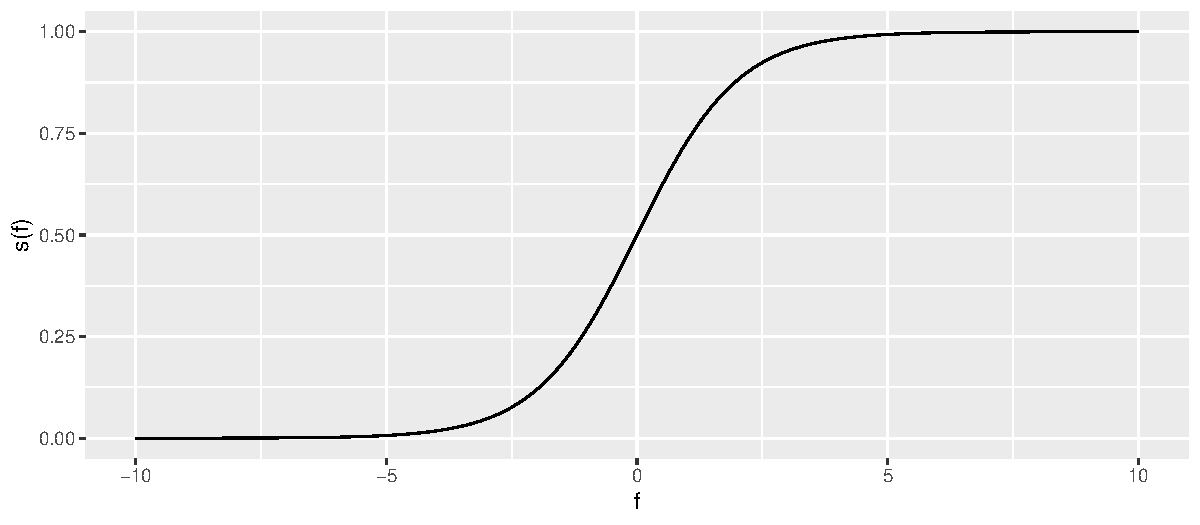
\includegraphics[width=0.95\textwidth]{figure/reg_class_log_1} 

}



\end{knitrout}

\framebreak
The intercept shifts $s(f)$ horizontally $s(\theta_0 + f) = \frac{\exp(\theta_0 + f)}{1+\exp(\theta_0 + f)}$
\begin{knitrout}\scriptsize
\definecolor{shadecolor}{rgb}{0.969, 0.969, 0.969}\color{fgcolor}

{\centering 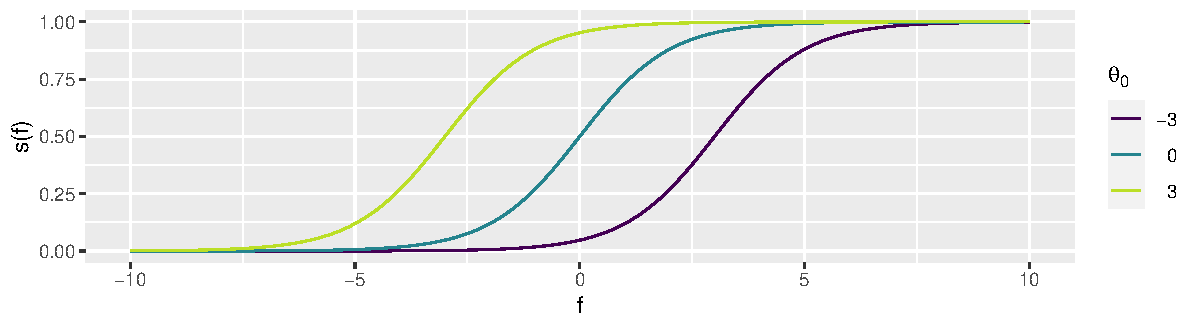
\includegraphics[width=0.95\textwidth]{figure/reg_class_log_2}  

}



\end{knitrout}

Scaling $f$ like $s(\alpha f) = \frac{\exp(\alpha f)}{1+\exp(\alpha f)}$: controls the slope and direction.
\lz
\begin{knitrout}\scriptsize
\definecolor{shadecolor}{rgb}{0.969, 0.969, 0.969}\color{fgcolor}

{\centering 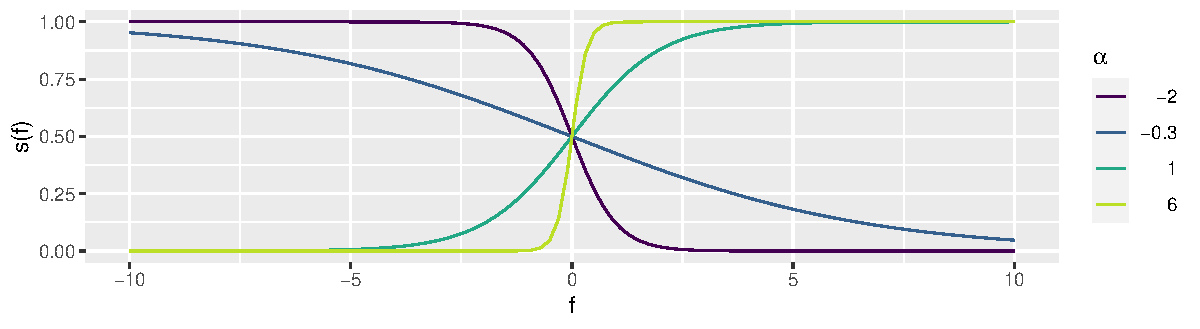
\includegraphics[width=0.95\textwidth]{figure/reg_class_log_3} 

}



\end{knitrout}

\end{vbframe}

\begin{vbframe}{Bernoulli / Log loss}

We need to define a loss function for the ERM approach:

\begin{itemize}
  \item $\Lpixy = -y\ln(\pix)-(1-y)\ln(1-\pix)$
  \item Penalizes confidently wrong predictions heavily
  \item Called Bernoulli, log or cross-entropy loss 
  \item We can derive it from the negative log-likelihood of Bernoulli / Logistic regression model in statistics
  \item Used for many other classifiers, e.g., in NNs or boosting 
\end{itemize}


\begin{knitrout}\scriptsize
\definecolor{shadecolor}{rgb}{0.969, 0.969, 0.969}\color{fgcolor}

{\centering 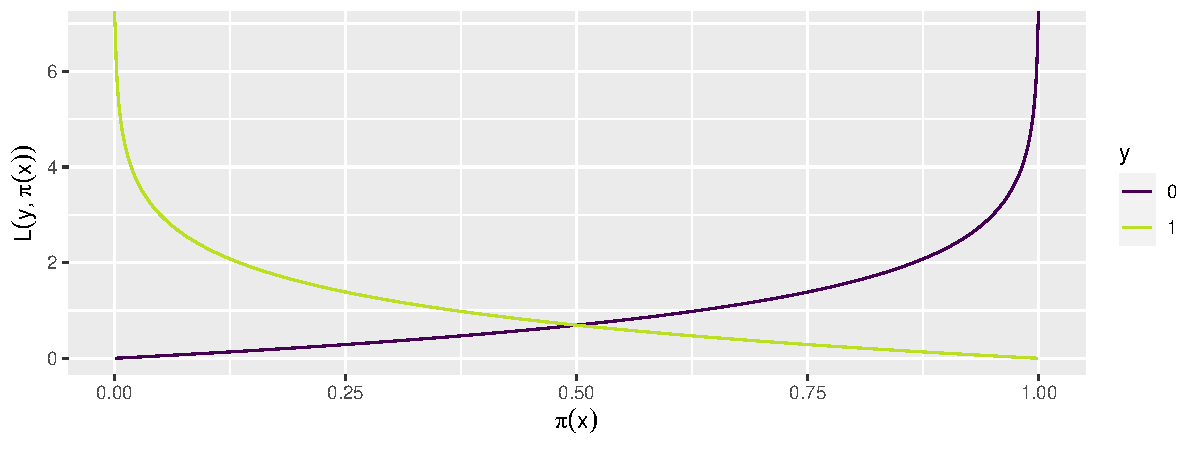
\includegraphics[width=0.95\textwidth]{figure/reg_class_log_4}  

}



\end{knitrout}

\end{vbframe}

\begin{vbframe}{Logistic Regression in 1D}
With one feature $\xv \in \R$. The figure shows data and $\xv \mapsto \pix$.

\begin{knitrout}\scriptsize
\definecolor{shadecolor}{rgb}{0.969, 0.969, 0.969}\color{fgcolor}

{\centering 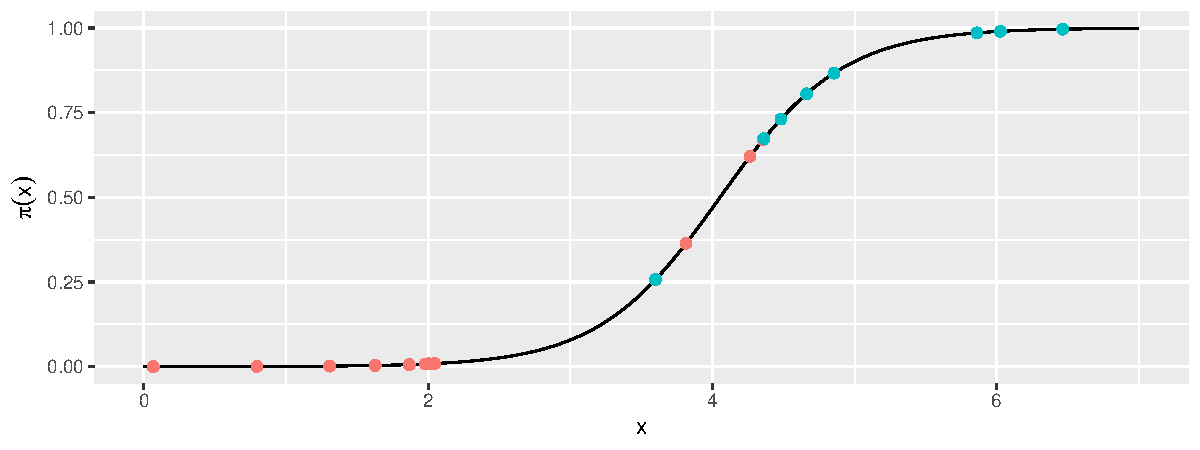
\includegraphics[width=0.95\textwidth]{figure/reg_class_log_5} 

}



\end{knitrout}
\end{vbframe}
\begin{vbframe}{Logistic Regression in 2D}

Obviously, logistic regression is a linear classifier, as $\pixt = s\left( \thetab^T \xv \right)$ 
and $s$ is isotonic.

\lz
\begin{knitrout}\scriptsize
\definecolor{shadecolor}{rgb}{0.969, 0.969, 0.969}\color{fgcolor}

{\centering 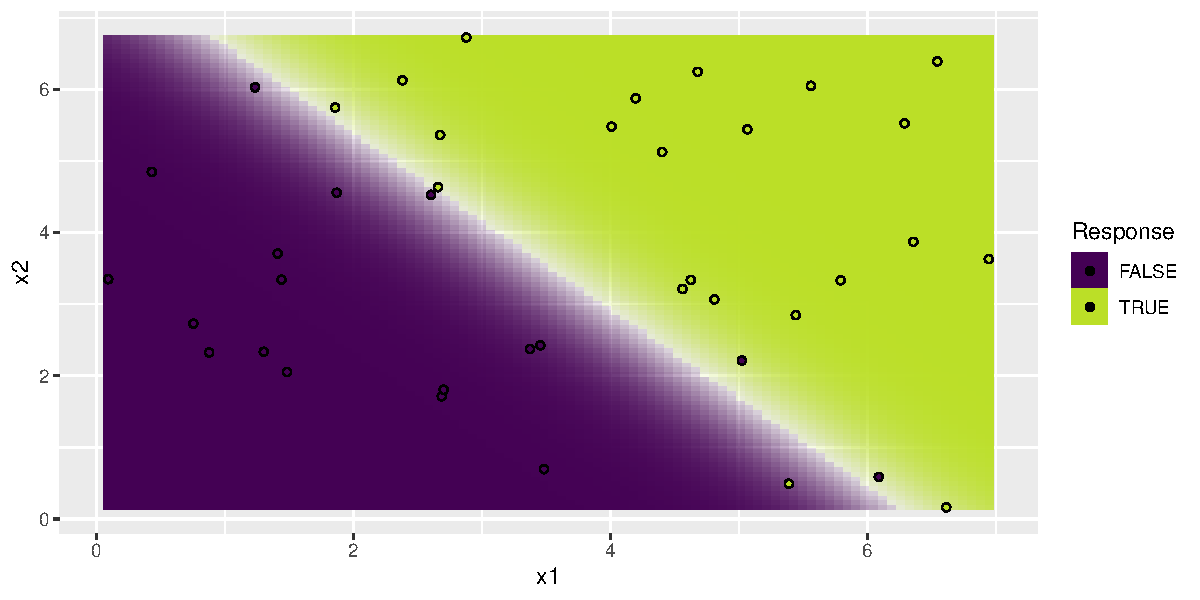
\includegraphics[width=0.95\textwidth]{figure/reg_class_log_6}  

}



\end{knitrout}

\framebreak

\begin{columns}[T]
\begin{column}{0.5\textwidth}
  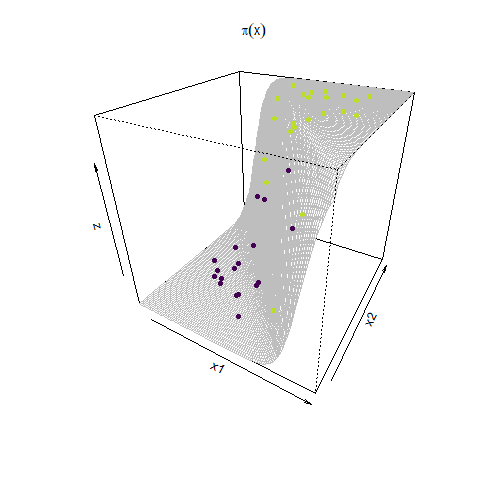
\includegraphics[width=\textwidth]{figure_man/logreg-2vars-surface.png}
\end{column}
\begin{column}{0.5\textwidth}
\begin{knitrout}\scriptsize
\definecolor{shadecolor}{rgb}{0.969, 0.969, 0.969}\color{fgcolor}

{\centering 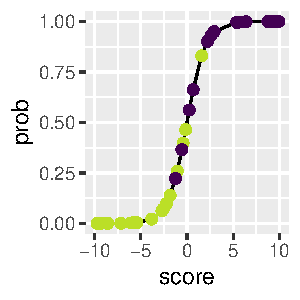
\includegraphics[width=0.95\textwidth]{figure/reg_class_log_7} 

}



\end{knitrout}
\end{column}
\end{columns}

% <<fig.width=2, fig.height=2>>=
% x1 = seq(-1, 8, by = 0.1)
% dfn = expand.grid(x1, x1)
% names(dfn) = c("x1", "x2")
% dfn$prob = predict(m, newdata = dfn)
% dfn$score = predict(mm, newdata = dfn)
% z = matrix(dfn$prob, nrow = length(x1))
% res = persp(x1, x1, z, phi = 30, theta = 30,
%   xlab = "x1", ylab = "x2",
%   main = expression(pi(x)), border = "grey"
% )
% cols = viridisLite::viridis(2, end = .9)
% mypoints = trans3d(df$x1, df$x2, df$prob, pmat = res)
% points(mypoints, pch = 19, col = cols[as.numeric(df$y) + 1])
% @ 


% \framebreak 

% \begin{center}
  % 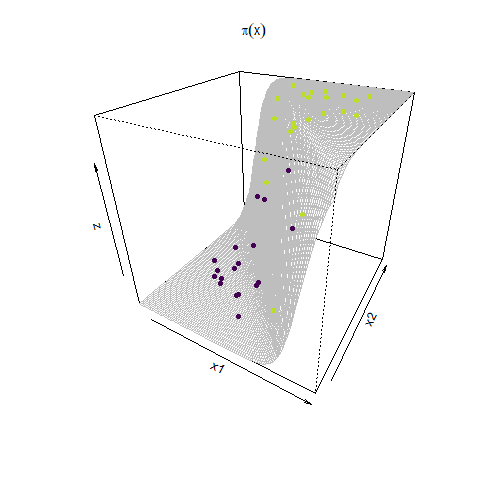
\includegraphics[width=0.4\textwidth]{figure_man/logreg-2vars-surface.png}
% \end{center}


\end{vbframe}


% \begin{vbframe}{Logistic Regression}

% \textbf{Multivariate logistic regression} combines the hypothesis space of linear functions 

% \vspace*{-0.3cm}

% \begin{eqnarray*}
%   \Hspace = \left\{f: \Xspace \to \R ~|~\fx = \thx \right\}
% \end{eqnarray*}

% with the \textbf{logistic loss}

% \vspace*{-0.2cm}

% \begin{eqnarray*}
%   \Lxy = \log \left[1 + \exp \left(-y\fx\right)\right].
% \end{eqnarray*}

% We transform scores into probabilities by 

% $$
% \pix = \P(y = 1 ~|~\xv) = s(\fx) = \frac{1}{1 + \exp(- \fx)},
% $$

% with $s(.)$ being the logistic sigmoid function as introduced in chapter 2.

% \framebreak 

% As already shown before, an equivalent approach that directly outputs probabilities $\pix$ is minimizing the \textbf{Bernoulli loss} 

% \begin{eqnarray*}
% \Lpixy = -y \log \left(\pix\right) - (1 - y) \log \left(1 - \pix\right)
% \end{eqnarray*}

% for $\pix$ in the hypothesis space

% \begin{eqnarray*}
%   \Hspace = \left\{\pi: \Xspace \to [0, 1] ~|~\pix = s(\thx)\right\}
% \end{eqnarray*}

% with $s(.)$ again being the logistic function. 

% \end{vbframe}

% \begin{vbframe}{Logistic Regression: Discriminant functions and decision boundary}

% Logistic regression gives us a \textbf{linear classifier}. 

% In order to minimize the loss (misclassification), we should predict $y=1$ if

% $$
% \pixt = \frac{\exp(\thx)}{1+\exp(\thx)} \ge 0.5,
% $$

% which is equivalent to
% $$
% \thx \ge 0 \implies y = 1.
% $$


% \lz 

% If we apply $g(y) = \log \left(\frac{y}{1 - y}\right)$ (which is a monotone, rank preserving function) on $\pix = \frac{1}{1 + \exp(-\thetab^\top \xv)}$, we get

% \begin{footnotesize}
% \begin{eqnarray*}
%   g(\pix) &=& g\left(\pix\right)\\
%   &=& \log\left(\pix)\right) - \log \left(1 - \pix\right) \\ &=& - \log (1 + \exp(- \fx)) - \log \left(1 - \frac{1}{1 + \exp(-\fx)}\right)\\
%   &=& - \log (1 + \exp(- \fx)) - \log \left(\frac{\exp(-\fx)}{1 + \exp(-\fx)}\right) \\
%   &=& - \log (1 + \exp(- \fx)) - \log \left(\exp(-\fx)\right) + \log\left(1 + \exp(-\fx)\right)\\
%    &=& \fx = \thx.
% \end{eqnarray*}
% \end{footnotesize}

% $\fx = \thx$ is the discriminant function of logistic regression and $\fx = \thx = 0$ represents the decision boundary, which is a \textbf{hyperplane} in the $p$ dimensional space. 

% \lz  

% The discriminant function can be interpreted as \textbf{log-odds ratio}: 

  % $$ \log \dfrac{\pix}{1-\pix} = \log \dfrac{\P(y = 1 ~|~ \xv)} {\P(y = 0 ~|~ \xv)} = \thx
  % = \fx.
  % $$
 

% \framebreak 

% <<logreg-plot, echo=FALSE, eval = FALSE, include = FALSE>>=
% n = 30
% set.seed(1234L)
% tar = factor(c(rep(1L, times = n), rep(2L, times = n)))
% feat1 = c(rnorm(n, sd = 1.5), rnorm(n, mean = 2, sd = 1.5))
% feat2 = c(rnorm(n, sd = 1.5), rnorm(n, mean = 2, sd = 1.5))
% bin.data = data.frame(feat1, feat2, tar)
% bin.tsk = makeClassifTask(data = bin.data, target = "tar")
% plotLearnerPrediction("classif.logreg", bin.tsk) + 
%   scale_f_d()
% @

% \end{vbframe}


\begin{frame}{Summary}
% \lz

\textbf{Hypothesis Space:} 
\begin{eqnarray*}
  \Hspace = \left\{\pi: \Xspace \to [0,1] ~|~\pix = s(\thx) \right\}
\end{eqnarray*}

\lz

\textbf{Risk:} Logistic/Bernoulli loss function.

\begin{eqnarray*}
  \Lpixy = -y\ln(\pix)-(1-y)\ln(1-\pix)
  % \Lxy = \log \left[1 + \exp \left(-y\fx\right)\right].
\end{eqnarray*}

\lz


\textbf{Optimization:} Numerical optimization, typically gradient based methods.

% We transform scores into probabilities by 

% $$
% \pix = \P(y = 1 ~|~\xv) = s(\fx) = \frac{1}{1 + \exp(- \fx)},
% $$

% with $s(.)$ being the logistic sigmoid function as introduced in chapter 2.

\end{frame}

\endlecture

\end{document}
